\chapter{Project Planning}\label{projPlan}
%Project plan and how it evolved (present the original plan and explain how it changed and why during the project)

The kick-off meeting was very important to make a plan for the project and take the most important
decisions concerning the implementation and development of the code.
First of all we agreed on using plain Java 13 (without the use of a simulator) because we
wanted to implement all the protocols and packets from scratch in order to have a deeper
understanding of the proposed task.\\
We also determined to implement IPv6 as network layer protocol since it has simpler fields with respect to IPv4 and
it's very important to get a better knowledge of it in the prospect of a future widespread use. In addition, we were
also open to do a dual-stack implementation in case we would have enough time (but it was not the case).

Thanks to our software engineering experience we were able to subdivide the main task in
subtasks and we put milestones and preferred deadlines for each of them, trying to predict
the amount of working hours required.\\
The work was split between the team members in the following way:
\begin{itemize}
    \item Simulator and infrastructure, Layer 2, Project management (Stephan)
    \item IPv6 (excluding routing) and TCP (Filippo)
    \item Routing and BGP (Mirko and Gabriele)
\end{itemize}

The first main step was to define almost all the interfaces that we would have need to implement.
In this way we could have a skeleton of the final product and we were able to call functions
or create objects that in reality were not implemented yet.
Moreover, almost each class has been accompained with some JUnit tests in order to verify
the correctness of the implementation and perform bug fixing module by module.

A detailed plan about tasks' splitting and the proposed deadlines is shown in figure ...

%\begin{figure}[h]
 %   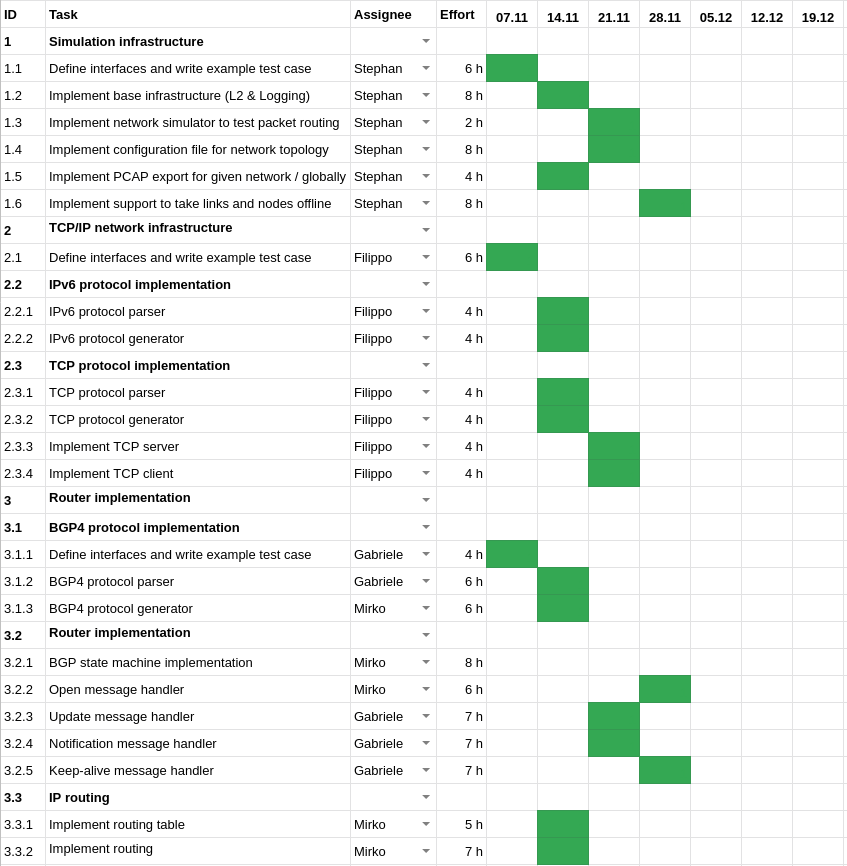
\includegraphics[width=\textwidth]{first_meeting.png}
 %   \caption{First week plan}
%\end{figure}

We managed to follow quite well the plan that we did at the beginning but we slightly
adapted it from time to time.
Very important for future debugging purposes was the implementation of a PCAP exporter
in order to verify the correctness of created packets using Wireshark.

\section{Week 1 \& 2}
At the end of the second week of work these were the results:

\begin{itemize}
    \item Simulation infrastructure (done)
    \item Layer 2 simulation based on Ethernet (done)
    \item PCAP export for all traffic (done)
    \item IPv6 packet parser \& generator (done)
    \item TCP datagram parser \& generator (done)
    \item BGP4 message parser \& generator (70 \%)
    \item IP routing table \& routing (60 \%)
\end{itemize}

For the week 3 we planned to implement end-to-end connection using TCP, dynamic routing
using BGP and the possibility of loading custom based scenarios.
To go more into the details:

\begin{itemize}
    \item Simulator: Load custom scenarios from files
    \item Simulator: Allow possibility to enable/disable links and nodes at runtime
    \item Finish IP routing (week 2 task)
    \item TCP server and client implementation
    \item BGP state machine
    \item BGP open, update, notification message handlers
\end{itemize}

\section{Week 3}
In this week Filippo joined Stephan in the implementation of the simulator and
core networking.

The results obtained at the end of the week are the following:

\begin{itemize}
    \item Bug fixing of previous tasks (done)
    \item BGP4 message parser \& generator (80 \%)
    \item implementation of longest prefix match algorithm (done)
    \item Simulator: Load customer scenarios from files (done)
    \item Simulator: Allow possibility to enable/disable links and nodes at runtime (moved to next week)
    \item TCP server \& client implementation (20 \%)
    \item BGP state machine (50 \%)
    \item BGP open, update, notification message handlers (moved to next week)
    \item Static routing (done)
\end{itemize}

